\documentclass[paper.tex]{subfiles}

\begin{document}


\section{Proof that $\mathcal{V}$ is a universal template}

In this section we outline the proof given in full detail in~\cite{Ghrist1996} that $\V$ (shown in figure~\ref{fig:universal}) is a universal template. Details will inevitably be omitted but our goal in this exposition is to straddle the line between
the full proof and the very high-level outline given in~\cite{knottyode}, giving a concise and readable exposition that gets at the essence of the proof.

The essential idea is to find a special set of templates which have a special property that forces them to support all braids as orbits, and then to show that these templates can be found in $\V$. Since all knots and links
can be realized as a braid, this immediately implies that $\V$ is universal. The last step of showing that the special braid-supporting templates can found in $\V$ is the most difficult by far and where we will have to do the
most hand-waving. Nonetheless, we will try to capture the essence.

\begin{figure}[h]
  % not sure where to put this, but not here
  \centering
  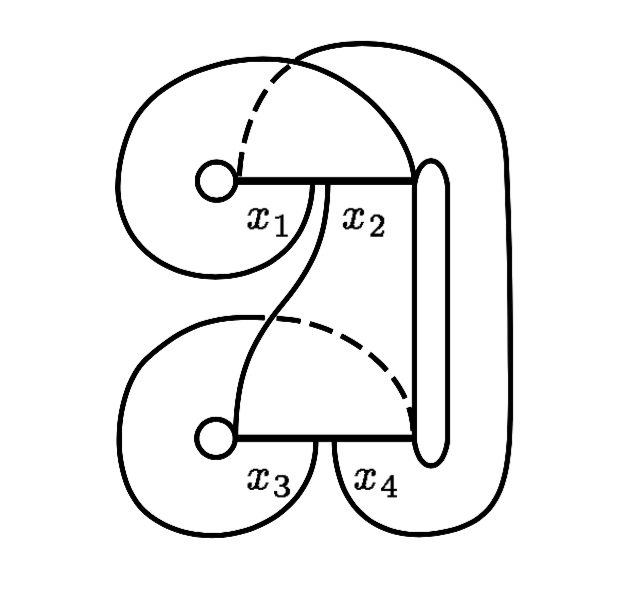
\includegraphics[width=0.5\textwidth]{universal.png}
  \caption{The universal template, reproduced from~\cite{knottyode}}\label{fig:universal}
\end{figure}

\subsection{Braids and the theorem of Alexander}

Recall that a braid is a collection of $P$ disjoint simple closed curves in a standardly embedded torus such that every cross-section of the torus intersects the braid in exactly $P$ points.
Braids have a natural identification as a permutation on $P$ elements, which is the property we exploit. In a landmark paper~\cite{Alexander1923}, Alexander proved the following theorem which provides the crucial connection
between braids and links.

% we exploit it since each permutation can be written as the product of exchanges

\begin{thm}[Alexander 1923]
  Each knot or link is isotopic to some closed braid on $P$ strands for some $P$
\end{thm}

\subsection{The templates $\W_q$}

The family of templates $\set{\W_q}$ shown in figure~\ref{fig:w_q} are those referred to earlier as the braid-supporting templates. $\W_1$ is identically $\V$ and increasing $q$ by one has the effect of adding
two \emph{ears} to one side. It's crucial that the ears alternate in `sign' as illustrated in the figure.

\begin{figure}[h]
  \centering
  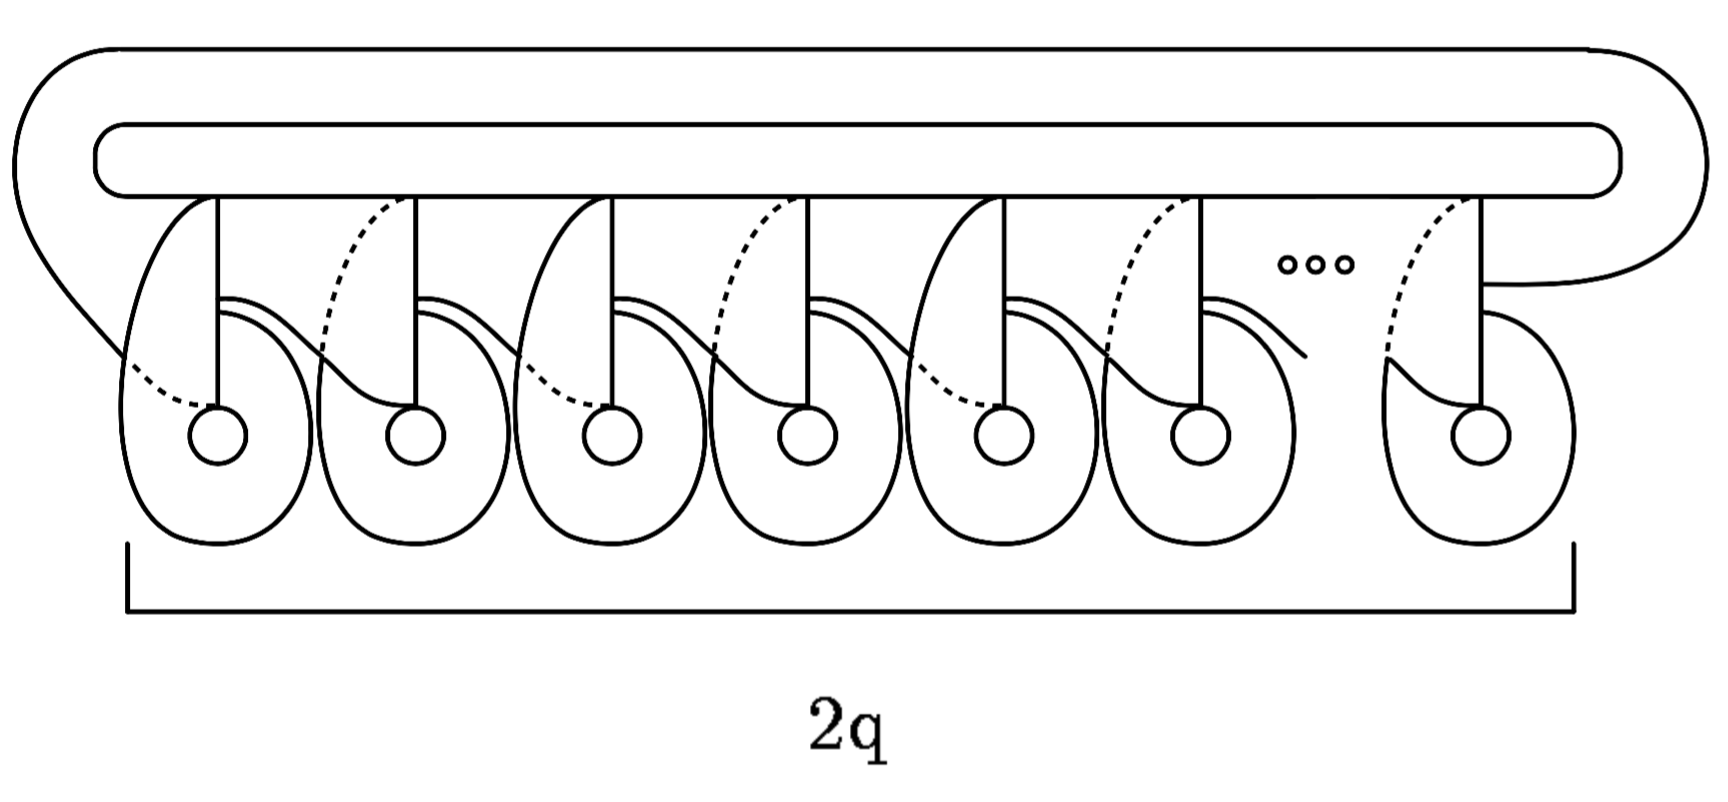
\includegraphics[width=0.8\textwidth]{w_q.png}
  \caption{The templates $W_q$, reproduced from~\cite{knottyode}}\label{fig:w_q}
\end{figure}


An isotopic copy of any closed braid exists as a set of periodic oribts on some $W_q$ for sufficently large $q$.


\subsection{Construct $\W_{q+1}$ from $\W_q$}

Start with renormalized $\W_1 \in \V$, and append a pair of ears to\dots

\subsection{Find $\W_q \subset \V$ for all $q$}

This is very tricky and will have to be very loosely sketched

This paper is referenced to prove this fact. (requires defining subtemplates; maybe that could be done in an earlier section)
https://www.math.upenn.edu/~ghrist/preprints/eraams.pdf

\end{document}
